\documentclass[12pt]{article}%
\usepackage[a4paper, top=2.5cm, bottom=2.5cm, left=2.2cm, right=2.2cm]
{geometry}
\usepackage{float}
\usepackage{graphicx}
\usepackage{listings}
\restylefloat{table}

%---------------------------------------------------------------------------
\begin{document}
\title{Switcher}
\author{Ashley J. Robinson}
\date{\today}
\maketitle
%---------------------------------------------------------------------------
\section{Introduction}

The task is to design and build a switch mode power supply (SMPS) which will operate in boost and buck mode. The controller will contain a selection of menu options allowing the user to control as many features as possible of the SMPS operation. The software running on the controlling processor must consist of no more than 1024 bytes of machine code.

\subsection{Processor selection}

The chosen processor is a \textbf{Silicon Labs C8051F850-C-GU} which uses the 8051 architecture. An 8051 processor is a good choice for a code size reduction exercise as there are many thoroughly tested compilers available. The Keil c51 compiler will be used to generate assembly for this project.

\section{Hardware}

A soldering iron and solder is required to build the switcher hardware. The schematic is held in Figure \ref{fig:sch} along with the BoM in Table \ref{tab:bom}. Photos of the top and bottom of the strip board build are contained in Figures \ref{fig:top} and \ref{fig:bot}. Note the visible modification to the development board is not required to replicated the design however \textbf{R5, R6 and R9 must be removed from the board development board}.

\subsection{Schematic}

\begin{figure}[H]
	\centering
  	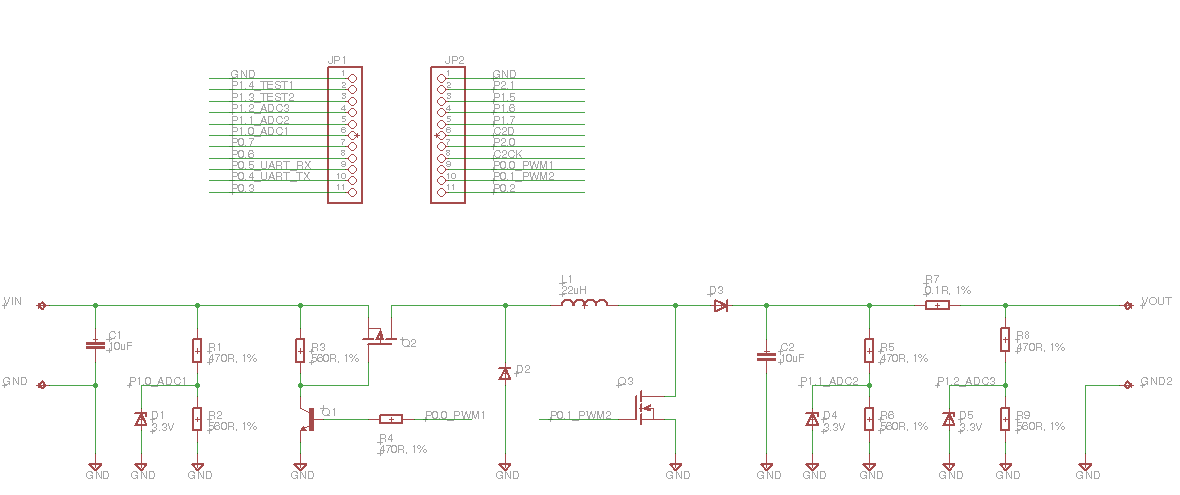
\includegraphics[width=16cm]{sch.png}
  	\caption{Schematic.}
  	\label{fig:sch}
\end{figure}

\subsection{Bill of Materials (BoM)}


\begin{table}[H]
   \centering
   \caption{BoM}
   \label{tab:bom}
   \begin{tabular}{|p{2.5cm}|p{1.2cm}|p{7cm}|p{5cm}|}
   \hline
      	\textbf{Designator}        	& 	\textbf{Value}	&	\textbf{Manufacturer}   		&  	\textbf{Manufacturer Part Number}	\\ \hline
	C1,C2				&	10uF			&	 MULTICOMP				&	MCGPR25V106M5X11			\\ \hline
	D1,D4,D5			&	3.3V			&	ON SEMICONDUCTOR		&	1N5333BG					\\ \hline
	D2,D3				&				&	TAIWAN SEMICONDUCTOR	&	SR1504					\\ \hline
	JP1,JP2			&				&	AMPHENOL FCI	&	77311-401-36LF					\\ \hline
	L1				&	22uH			&	PANASONIC 	&	ELC08D220E			\\ \hline
	Q1				&				& 	MULTICOMP	                              &      BC337		\\ \hline
	Q2				&			&	FAIRCHILD SEMICONDUCTOR	&	FQP27P06		\\ \hline
	Q3				&		&	FAIRCHILD SEMICONDUCTOR	&	FQP30N06L	\\ \hline
	R1,R4,R5,R8		&	470$\Omega$		&	MULTICOMP	&	MF12 470R	\\ \hline
	R2,R3,R6,R9		&	560$\Omega$		&	MULTICOMP	&	MF12 560R	\\ \hline
	R7		&	0.1$\Omega$		&	VISHAY	&  LVR01R1000FE12	\\ \hline
	Strip board		&		&	KEMO & ELECTRONIC	E012	\\ \hline
	Dev board		&		&	SILICON LABS	&  LTOOLSTICK850DC-UG	\\ \hline

   \end{tabular}
\end{table}


\subsection{Strip board}

\begin{figure}[H]
	\centering
  	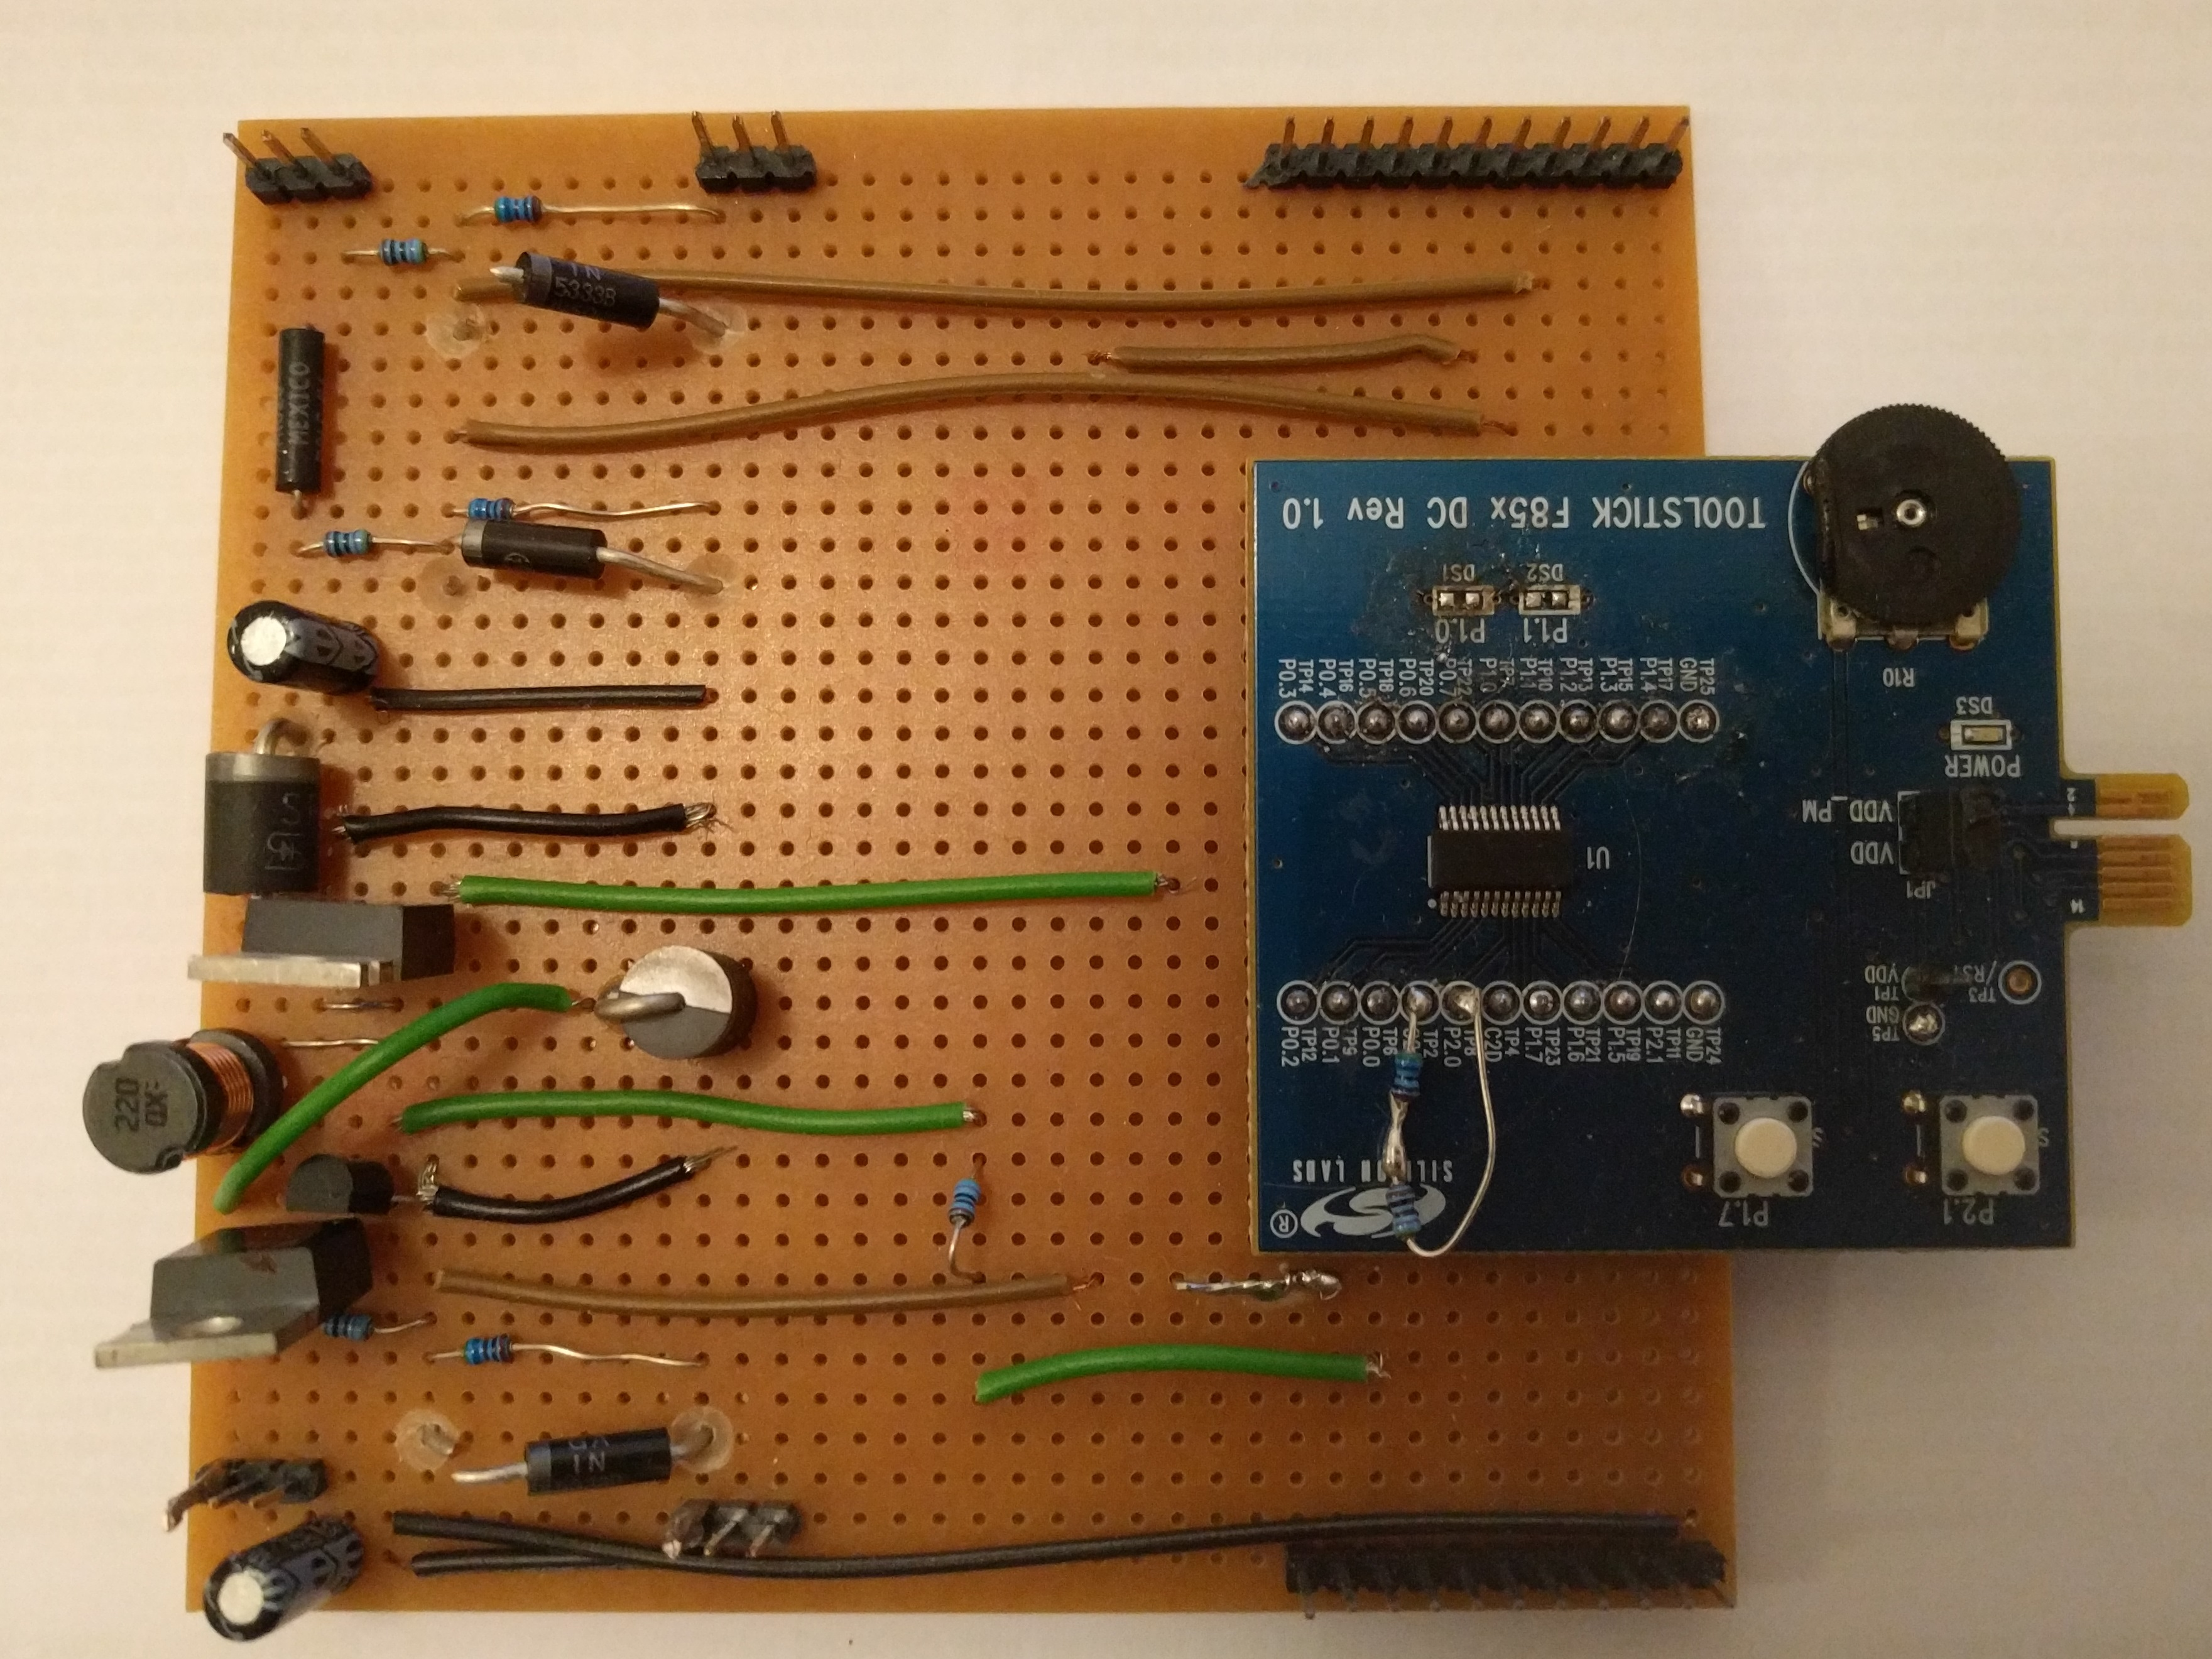
\includegraphics[width=16cm]{top.jpg}
  	\caption{Strip board top side.}
  	\label{fig:top}
\end{figure}

\begin{figure}[H]
	\centering
  	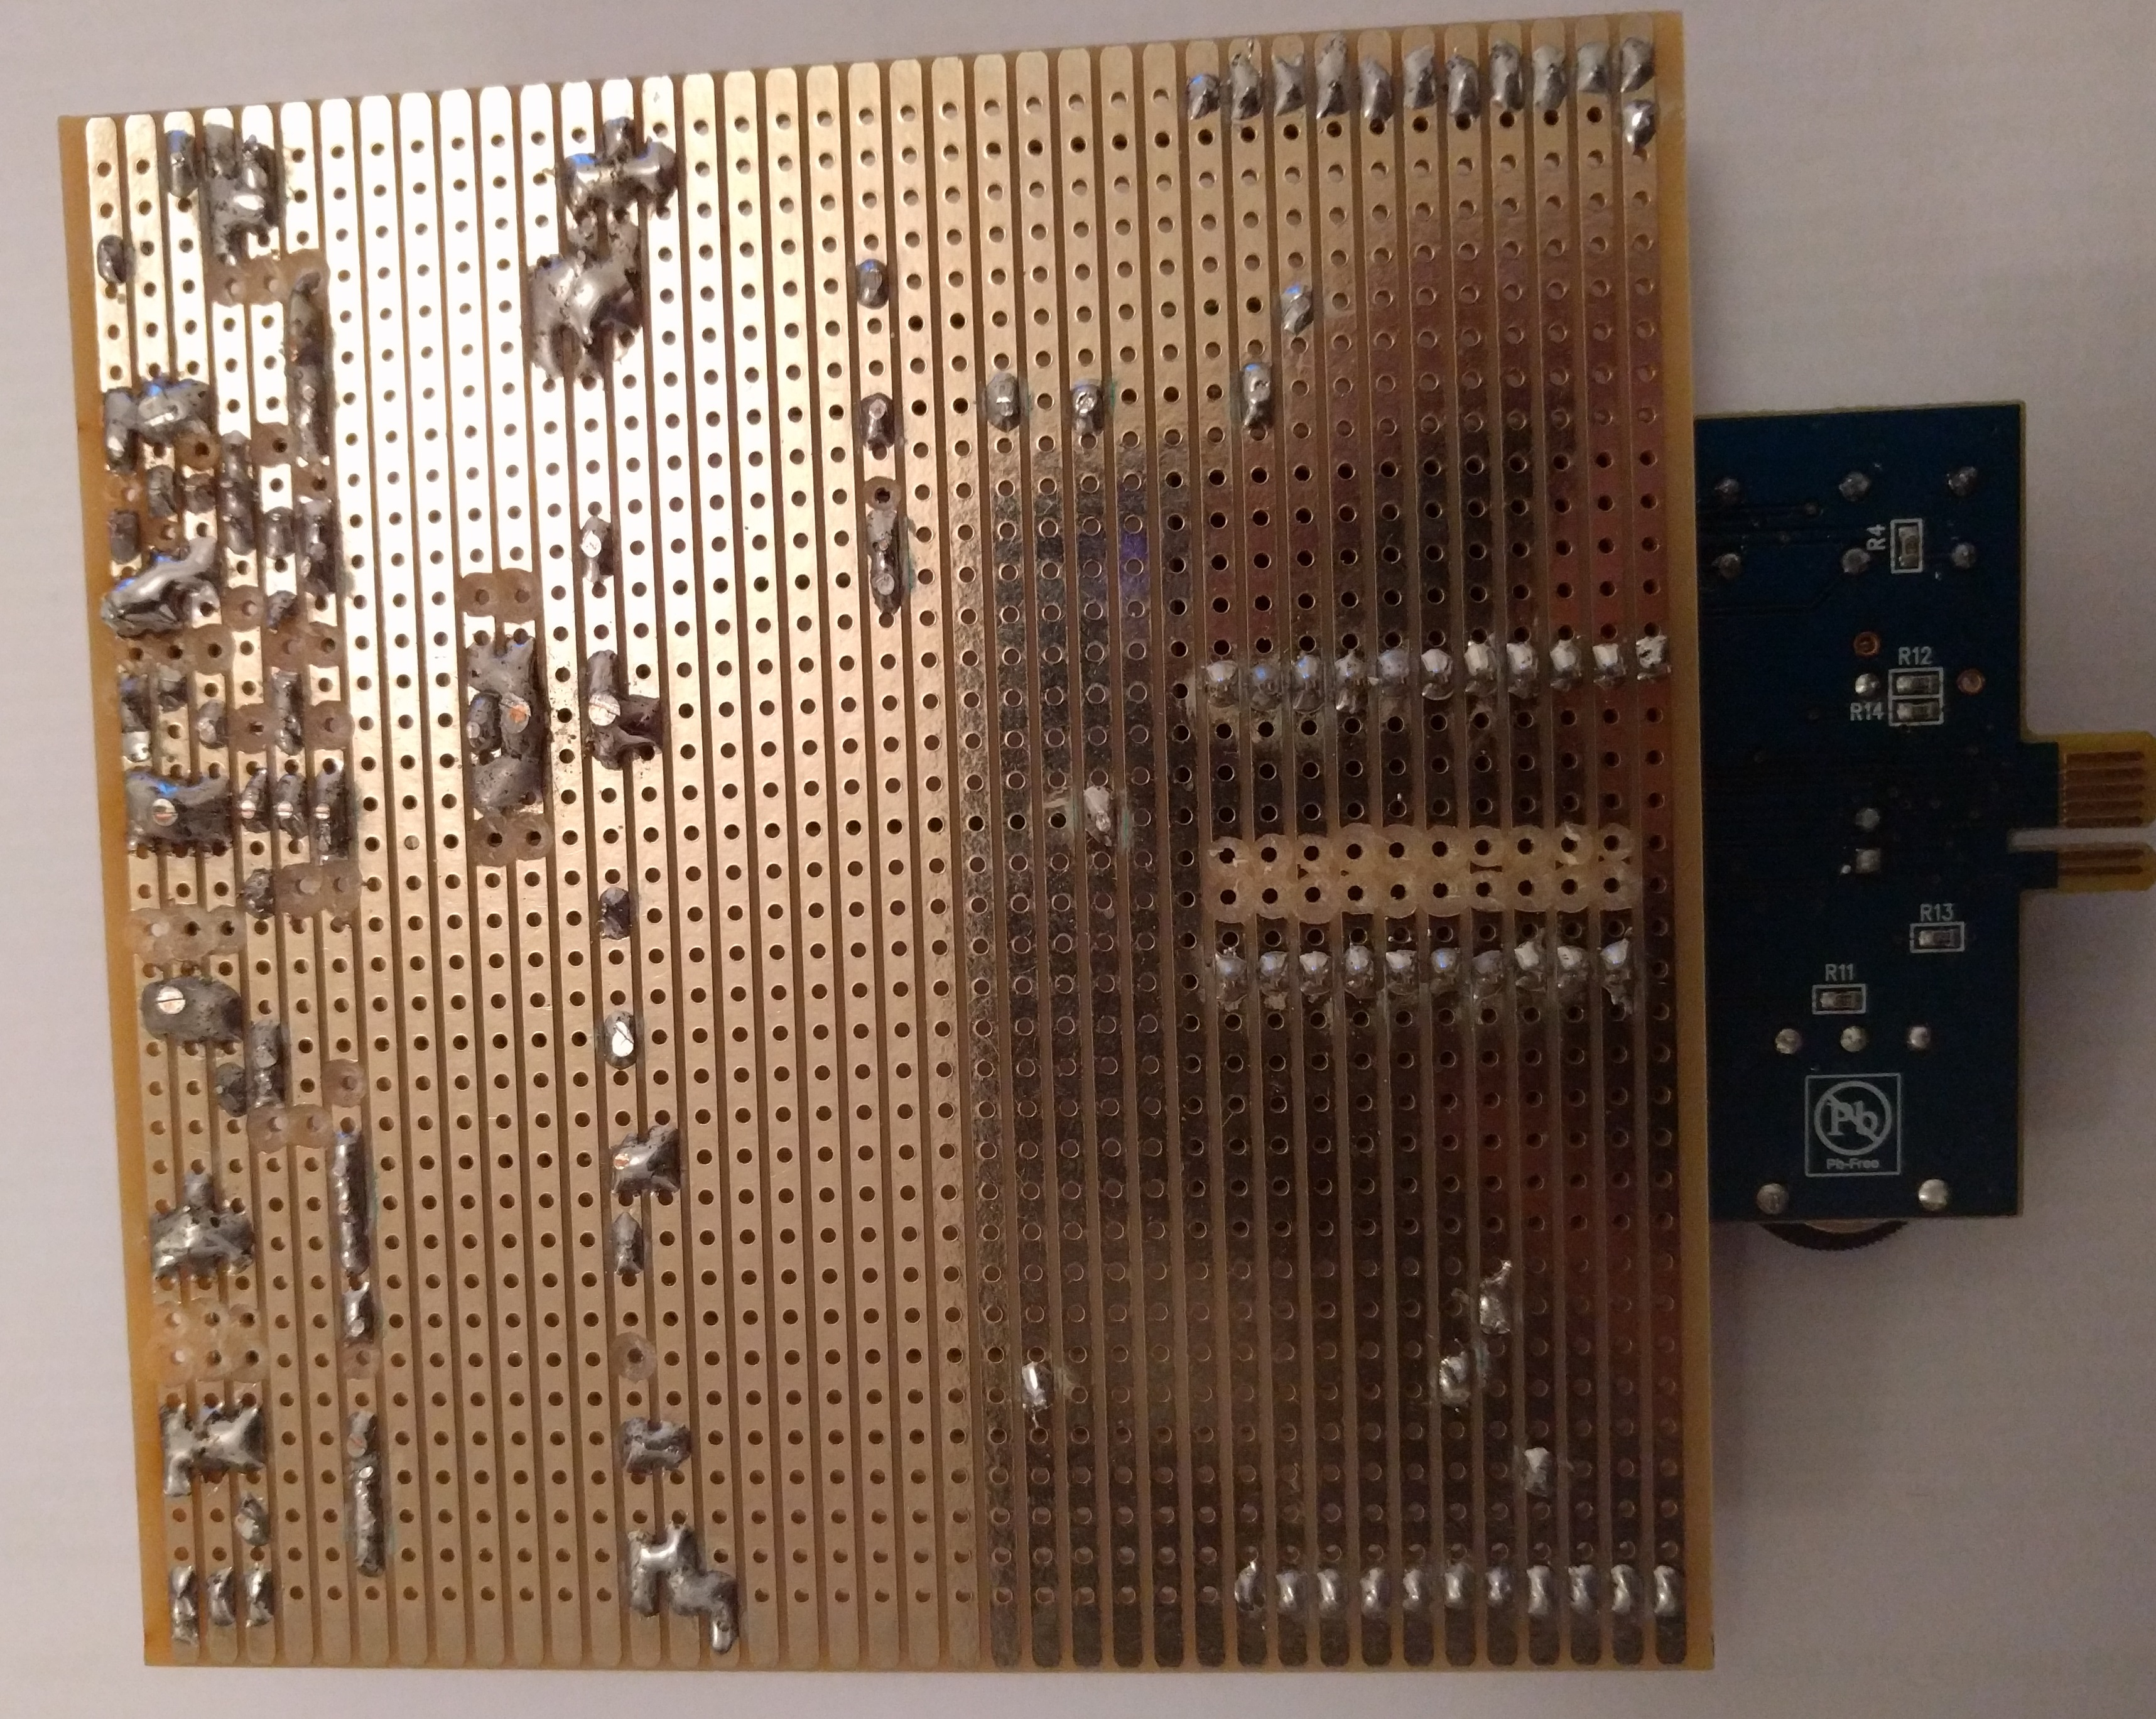
\includegraphics[width=16cm]{bot.jpg}
  	\caption{Strip board bottom side.}
  	\label{fig:bot}
\end{figure}

\section{Software}

\subsection{Peripherals}

\subsubsection{Analogue to Digital Converters (ADCs)}

A single ADC is multiplexed to measure three voltages on the board. 

\subsubsection{Universal Asynchronous/Synchronous Transceiver (UART)}

Transmission from the microcontroller happens through \textbf{uartLoadOut} which adds to the \textbf{8 byte} buffer and is then unloaded from a timer. The input is not interrupt driven and is handled in the main loop using a \textbf{5 byte} buffer that is enough to contain the longest command.

\subsubsection{Programmable Counter Array (PCA)}

The Pulse Width Modulation (PWM) is controlled from the counter array. The output runs at approximately 96KHz with 8 bits to control the duty cycle. A high resolution for control would be favorable for this application but the frequency achieved in 16-bit mode is far too low for this application.

\subsubsection{Timers}

\textbf{Timer 0} is used as baud rate generation for the UART. \textbf{Timer 2} is used to trigger an Interrupt Service Routine (ISR) which runs at 4KHz. The ISR controls the UART transmission, sampling of the ADC, running the controller and finally setting the PWM.

\subsection{Operation}

A brief description of the software operation is contained in Figure \ref{fig:overview} and the full code in Listing \ref{main.c}.

\begin{figure}[H]
	\centering
  	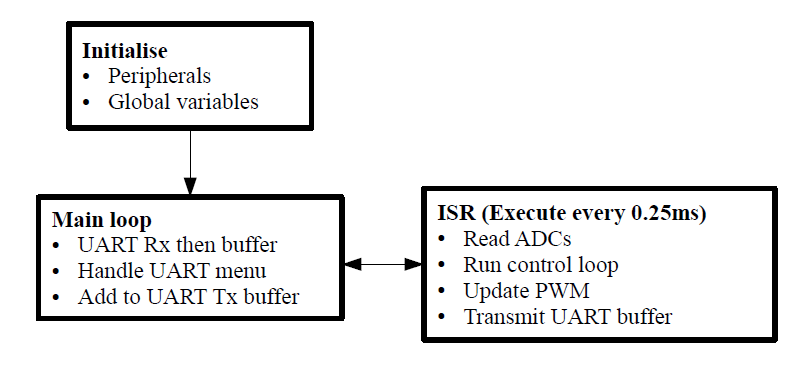
\includegraphics[width=12cm]{code.png}
  	\caption{Software overview.}
  	\label{fig:overview}
\end{figure}



\subsection{UART Menu}

The baud rate of the UART is 115200 with 8 data bits, no parity or control flow. The commands in Table \ref{tab:menu} reference the single characters for the menu and amount of the data to be exchanged.

\begin{table}[H]
   \centering
   \caption{UART menu}
   \label{tab:menu}
   \begin{tabular}{|p{4cm}|p{1.2cm}|p{1.8cm}|p{1.8cm}|p{5cm}|}
   \hline
      \textbf{Command}              & \textbf{Char}   &  \textbf{Send numbers}   &  \textbf{Return numbers}  &  \textbf{Notes}\\ \hline
      Enable                        & g               &  0                       &  0                        &  0                        \\ \hline
      Disable                       & s               &  0                       &  0                        &  0                        \\ \hline
      Read ADC1                     & x               &  0                       &  4                        &  Result in mV                         \\ \hline
      Read ADC2                     & y               &  0                       &  4                        &  Result in mV                         \\ \hline
      Read ADC3                     & z               &  0                       &  4                        &  Result in mV                         \\ \hline
      Read PWM duty                    & d               &  0                       &  4                        &  Percent = Result /2.55                         \\ \hline
      Read output current           & c               &  0                       &  4                        &  Result in mA              \\ \hline
      Set output voltage            & v               &  4                       &  0                        &  Send value in mV         \\ \hline
      Set input voltage upper limit & h               &  4                       &  0                        &  Send value in mV             \\ \hline
      Set input voltage lower limit & l               &  4                       &  0                        &  Send value in mV         \\ \hline
      Read set output voltage            & a               &  0                      &  4                       &  Result value in mV         \\ \hline
      Read set input voltage upper limit & m               &  0                       &  4                        &  Result in mV             \\ \hline
      Read set input voltage lower limit & n              &  0                       &  4                        &  Result in mV         \\ \hline
   \end{tabular}
\end{table}




\subsection{Assembly analysis}

The following sections of code are library functions inserted by the compiler implicitly to facilitate some more complex operations. A total of 146 lines of assembly are inserted for the implicit functions; not including any extra code to build stack frames, etc.

\subsubsection{ADC scaling}

Listing \ref{adc0} is a line of code operating on a 32 bit signed integer and invokes listing \ref{limul} and \ref{ulshr}. The purpose of this operation is to cast the voltage recorded by the ADC to a representation in mV. It is possible for the target voltage to be translated instead but this would still require the same piece of code. The 12 bit output but the ADC must be multiplied 5.926 as to represent the voltage at the top of the potential divider. Fixed bit multiplication followed by a shift operation removes the need for a floating point operation but yields the same result. The value of the potential dividers can be changed to improve the operation required. The additional lines of assembly total 57 from using this operation.

\lstset{
  caption=ADC, 
  basicstyle=\footnotesize, frame=tb,basicstyle=\fontsize{6}{7}\ttfamily,
  xleftmargin=.2\textwidth, xrightmargin=.2\textwidth,
label=adc0
}
\begin{lstlisting}
return (((U32)ADC0)*SCALE_MUL) >> 10;
\end{lstlisting}







\subsubsection{Division}

Division and modulus operations are contained in \ref{div} invoke the functions contained in \ref{udiv} which contains 62 lines of assembly. 

\lstset{
  caption=Division, 
  basicstyle=\footnotesize, frame=tb,basicstyle=\fontsize{6}{7}\ttfamily,
  xleftmargin=.2\textwidth, xrightmargin=.2\textwidth,
label=div
}
\begin{lstlisting}
scale /= 10;

num = out / scale;

out %= scale;	
\end{lstlisting}


\subsubsection{Switch}

Using a case statement will generate different assembly from an if/else ladder. The function in Listing \ref{ccase} is used to control the switch statement and totals 27 lines of assembly.


\section{Testing}

The potential dividers constantly place the power supply under a load of $515\Omega$. To test both the UART interface anhd the switch mode functionality a small python script is used to create GUI to plot values in real time. The input and output voltages recorded by the microcontroller are contained in Figure \ref{fig:gui} and the actual values are contained in \ref{fig:scope}.

\begin{figure}[H]
	\centering
  	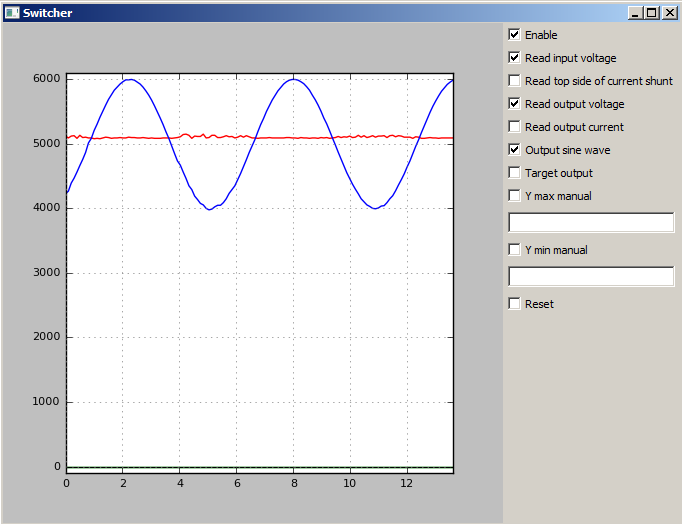
\includegraphics[width=12cm]{gui.png}
  	\caption{Sine wave output on GUI.}
  	\label{fig:gui}
\end{figure}

\begin{figure}[H]
	\centering
  	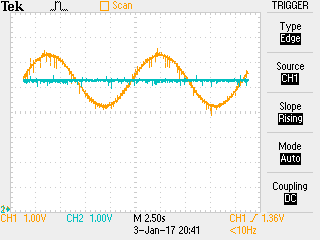
\includegraphics[width=12cm]{scope.png}
  	\caption{Sine wave output on scope.}
  	\label{fig:scope}
\end{figure}



\section{Conclusion}

The complete assembly in listing \ref{switcher.asm} is generated from the code in listing \ref{main.c}. The C code is contained within a single file and generates $950$ lines of assembler with an additional $3$ lines contained within the jump table and the jump on reset...

\begin{itemize}
  	\item \textbf{0x0000} Jumps straight to 0x0800
	\item \textbf{0x001B} Jump table entry TIMER1\_ISR(C:0BB6)
	\item \textbf{0x002B} Jump table entry TIMER2\_ISR(C:094C)
	\item \textbf{0x0800} First line of code generated from main.c
  	\item \textbf{0x0BB6} Final line of code generated from main.c
\end{itemize}

The Keil c51 compiler limits machine code generation to 2KB (not a problem) however it also limits the use of memory less than 2KB by always jumping to address $2048$ and then continuing with the compiled assembler. Excluding the first $2048$ is not completely fair because the jump on reset and the jump table would still exist. The highest vector used in the jump table is at address $43$ so assuming this is not optimised by the compiler the total code size comes to \textbf{993 bytes}.

\subsection{Code size over time}

The graph in \ref{fig:size} plots code size against discrete commits. Initial development is erratic, the size slowly grows as more features are added and eventually the code is optimised  back below the limit.

\begin{figure}[H]
	\centering
  	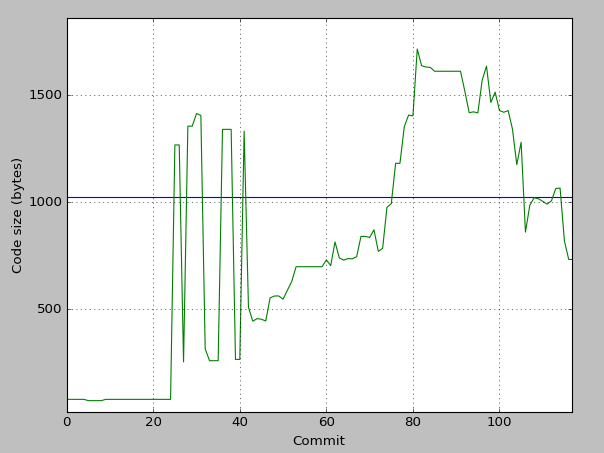
\includegraphics[width=12cm]{size.png}
  	\caption{Code size against commits.}
  	\label{fig:size}
\end{figure}


\subsection{Further work}

\begin{itemize}
  	\item Improve output current
	\item Replaced protection diodes with suitable parts
	\item Improve resolution of ADC to enable constant control
\end{itemize}

\section{Appendix}

\subsection{Code listings}

\lstset{
  caption=main.c, 
  basicstyle=\fontsize{6}{7}\ttfamily, frame=tb,
  xleftmargin=.05\textwidth, xrightmargin=.05\textwidth,
label=main.c, tabsize=4	
}
\lstinputlisting[language=C]{main.c}

\lstset{
  caption=Swicther.asm, 
  basicstyle=\footnotesize, frame=tb,basicstyle=\fontsize{6}{7}\ttfamily,
  xleftmargin=.2\textwidth, xrightmargin=.2\textwidth,
label=switcher.asm
}
\lstinputlisting{Switcher.asm}

\lstset{
  caption=LIMUL, 
  basicstyle=\footnotesize, frame=tb,basicstyle=\fontsize{6}{7}\ttfamily,
  xleftmargin=.2\textwidth, xrightmargin=.2\textwidth,
label=limul
}
\lstinputlisting{limul.asm}

\lstset{
  caption=ULSHR, 
  basicstyle=\footnotesize, frame=tb,basicstyle=\fontsize{6}{7}\ttfamily,
  xleftmargin=.2\textwidth, xrightmargin=.2\textwidth,
label=ulshr
}
\lstinputlisting{ulshr.asm}


\lstset{
  caption=IMUL, 
  basicstyle=\footnotesize, frame=tb,basicstyle=\fontsize{6}{7}\ttfamily,
  xleftmargin=.2\textwidth, xrightmargin=.2\textwidth,
label=imul
}
\lstinputlisting{imul.asm}


\lstset{
  caption=UDIV, 
  basicstyle=\footnotesize, frame=tb,basicstyle=\fontsize{6}{7}\ttfamily,
  xleftmargin=.2\textwidth, xrightmargin=.2\textwidth,
label=udiv
}
\lstinputlisting{udiv.asm}


\lstset{
  caption=CCASE, 
  basicstyle=\footnotesize, frame=tb,basicstyle=\fontsize{6}{7}\ttfamily,
  xleftmargin=.2\textwidth, xrightmargin=.2\textwidth,
label=ccase
}
\lstinputlisting{ccase.asm}



       
%---------------------------------------------------------------------------
\end{document}
